\chapter{Sensors and measurements}

\textbf{Author: Lukas Leskovar} 

The means of perceiving ones surrounding environment are a crucial part of any robotic system. This chapter aims to describe the need for interoceptive measurements aiding the different algorithms used within Autumn as well as any sensory equipment supporting such data acquisition. To this end the underlying principles and concepts behind the measurement techniques and  are illustrated.

\section{Motion Models}
Kinematic models in robotics are used for describing and planning state-transitions between consecutive robot poses. While Chapter \ref{chapter:slam} focuses on the theoretic basics of such models and how to build upon them, this section is going to focus on the practical concepts used in robot localization. To this end classical odometry as well as velocity based motion models are described.
To facilitate any equations later in this section the robot pose is described by its state vector 
\[
\begin{pmatrix}
	x \\
	y \\
	\theta \\
\end{pmatrix}
\] 
which defines its position as Cartesian coordinates and bearing as angular orientation $\theta$ in 2 dimensional space. 

\subsection{Odometry}
Ben-Ari and Mondada define this topic as follows: "Odometry—the measurement of distance—is a fundamental method used by robots for navigation.". \footcite{ben2017elements} 
When performing linear odometry, e.g. without taking orientation changes into consideration, this distance is calculated rather trivially by inferring it through measured time elapsed and the velocity of the robot proportionally to the motor power. 
Other systems however utilize wheel encoders to count the number of wheel rotations thus allowing for rather precise estimation of distance. 

With non-linear motion the distances $d_{l}$ and $d_{r}$ moved by the left and right wheel are unequal which requires the calculation of both updated position and bearing of the robot. 
Lets suppose a robot moved from position $\begin{pmatrix} x & y & \theta \end{pmatrix}$ to $\begin{pmatrix} x' & y' & \theta' \end{pmatrix}$ with a slight left turn caused by the right wheel turning faster than the left one. 
This scenario is depicted in Fig. \ref{fig:odom} with $\phi$ corresponding to the turn angle in radians, the radii $r_{l}, r_{c}, r_{r}$ describing the distance from the new position of the wheels and center to point P, the origin of the turn. 

For small angles these radii are approximately the same length as the distances $d_{l}, d_{c}$ and $d_{r}$, which allows for the turn angle to be calculated as follows:
\begin{align*}
	\phi &= \frac{d_{i}}{r_{i}}, & i &= l, r, c  
\end{align*}

However in practical scenarios these radii and the point P are unknown $\phi$ has to be calculated only using $d_{l}$, $d_{r}$ and b which corresponds to the distance between both robot wheels.

\begin{equation*}
	\begin{split}
		\phi r_{r} = d_{r} \\
		\phi r_{l} = d_{l} \\
		\phi r_{r} - \phi r_{l} = d_{r} - d_{l} \\
		\phi = \frac{d_{r} - d_{l}}{r_{r} - r_{l}} \\ 
		\phi = \frac{d_{r} - d_{l}}{b} \\
	\end{split}
\end{equation*}

To calculate the new coordinate positions the distance $d_{c}$ is computed:
\begin{equation*}
	d_{c} = \frac{d_{l} + d_{r}}{2}
\end{equation*}

The final pose is calculated as follows:

\begin{equation*}
	\begin{pmatrix}
		x' & y' & \theta'
	\end{pmatrix}
	= 
	\begin{pmatrix}
		-d_{c} \sin \phi & d_{c} \cos \phi & \theta + \phi
	\end{pmatrix}
\end{equation*}

Because the assumptions above only apply for small distances in any real-world systems such computations ought to be performed continuously. However due to uncertain measurements these calculations inherit some error which is added up over multiple iterations thus causing a slight drift in the output. This drift can be corrected using techniques discussed in Chapter \ref{chapter:slam}.

\begin{figure}
	\centering
	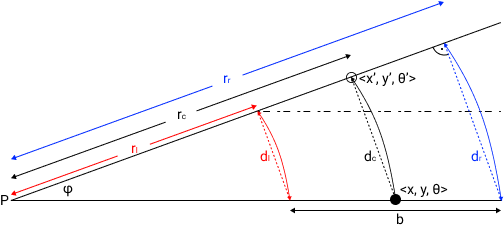
\includegraphics[width=0.8\linewidth]{img/odom}
	\caption{
		This diagram shows the geometry of how a slight turning can be calculated only using the distances $d_{l}$, $d_{r}$ and wheel offset b.
		The robot pose 
		$
			\begin{pmatrix}
				x &
				y &
				\theta 
			\end{pmatrix}
		$
		is associated with the center of the robot.
	}
	\label{fig:odom}
\end{figure}


\subsection{Inertial Measurement}

\subsection{Visual Inertial Odometry}


\section{Depth Sensing}

\subsection{Stereo Sensing}

\subsubsection{Projective Geometry}

\subsubsection{Homogenous Coordinates}

\subsubsection{ZED 1 vs ZED 2}

\subsection{LiDAR Depth Sensing}

\subsection{AI based depth sensing}


\section{Other Measurements}


\filbreak